\documentclass[a4paper, 12pt]{article}

\def\languages{english, french}

%%%%%%%%%%%%%%%%%%% Libraries

%%%%%%%%%% Packages

%%%%% Coding tools

\usepackage{comment}
\usepackage{xstring}

%%%%% Encoding

\usepackage[utf8]{inputenc}
\usepackage[T1]{fontenc}
\usepackage{eurosym}

%%%%% Languages

\ifx\languages\undefined
	\usepackage[english]{babel}
\else
	\usepackage[\languages]{babel}
\fi

\def\languagefile{./include/languages/\languagename.tex}
\InputIfFileExists{\languagefile}{}

%%%%% Style

\usepackage{geometry}
\usepackage{fancyhdr}
\usepackage[bottom]{footmisc}

\edef\restoreparindent{\parindent=\the\parindent\relax}
\usepackage[parfill]{parskip}

\usepackage{enumitem}
\usepackage{csquotes}
\usepackage{color}

%%%%% Others

\usepackage[framemethod=TikZ]{mdframed}
\usepackage[pdfusetitle]{hyperref}

%%%%%%%%%% Features

%%%%% Settings

\geometry{paper=a4paper,top=3.5cm,bottom=2.5cm,right=2.5cm,left=2.5cm}

\pagestyle{fancy}
\fancyhead[L]{}
\fancyhead[R]{\leftmark}
\fancyfoot[C]{\thepage}
\renewcommand{\headrulewidth}{0pt}

%\restoreparindent

%%%%% Commands

\newcommand{\romantableofcontents}{
	\newpage
	\pagenumbering{roman}
	\tableofcontents
	\newpage
	\pagenumbering{arabic}
}

%%%%%%%%%% Packages

\usepackage{inconsolata}
\usepackage{listings}

%%%%%%%%%% Features

%%%%% Commands

\newcommand{\Nstyle}[1]{
	\lstdefinestyle{N#1}{
		style=#1,
		%%%%%
		numbers=left
	}
}

\newcommand{\tbFstyle}[1]{
	\lstdefinestyle{tbF#1}{
		style=#1,
		%%%%%
		aboveskip=1.5em,
		frame=tb,
	}
}

\newcommand{\Fstyle}[1]{
	\lstdefinestyle{F#1}{
		style=#1,
		%%%%%
		aboveskip=1.5em,
		frame=single,
		framesep=0em,
		rulesep=0em,
		xleftmargin=0.75em,
		xrightmargin=0.75em,
		framexleftmargin=0.75em,
		framexrightmargin=0.75em,
		framextopmargin=0.5em,
		framexbottommargin=0.5em,
		%%%%%
		numbersep=1.25em
	}
}

\newcommand{\NtbFstyle}[1]{
	\tbFstyle{#1}
	\Nstyle{tbF#1}
}

\newcommand{\NFstyle}[1]{
	\Fstyle{#1}
	\lstdefinestyle{NF#1}{
		style=f#1,
		%%%%%
		xleftmargin=2.75em,
		framexleftmargin=2.75em,
		%%%%%
		numbers=left,
		numbersep=1em
	}
}

%%%%% Styles

\lstdefinestyle{default}{
	aboveskip=1em,
	breaklines=true,
	breakatwhitespace=true,
	columns=fixed,
	extendedchars=true,
	upquote=true,
	tabsize=4,
	%%%%%
	framerule=0.66pt,
	captionpos=b,
	%%%%%
	basicstyle=\footnotesize\ttfamily,
	numberstyle=\footnotesize\ttfamily,
	showstringspaces=false
}
\Nstyle{default}
\NFstyle{default}
\NtbFstyle{default}

\lstdefinestyle{monokai}{
	style=Fdefault,
	%%%%%
	backgroundcolor=\color[HTML]{272822},
	framerule=0em,
	%%%%%
	basicstyle=\footnotesize\ttfamily\color[HTML]{f8f8f2},
	numberstyle=\footnotesize\ttfamily\color[HTML]{272822},
	commentstyle=\color[HTML]{75715e},
	keywordstyle=[1]{\color[HTML]{f92672}},
	keywordstyle=[2]{\color[HTML]{A6E22E}},
	keywordstyle=[3]{\color[HTML]{ae81ff}},
	stringstyle=\color[HTML]{e6db74},
	%%%%%
	% otherkeywords={!,.,+,-,*,/,=,<,>,^,|,\&,OR,AND}
}

\lstdefinestyle{Nmonokai}{
	style=monokai,
	%%%%%
	xleftmargin=2.75em,
	framexleftmargin=2.75em,
	%%%%%
	numbers=left,
	numberstyle=\footnotesize\ttfamily\color[HTML]{f8f8f2},
	numbersep=1em
}

\lstdefinestyle{c}{
	language=C,
	style=default,
	%%%%%
	commentstyle=\color[HTML]{228B22},
	keywordstyle=\color[HTML]{0000FF},
	stringstyle=\color[HTML]{A020F0},
	emphstyle=\color[HTML]{0000FF},
	%%%%%
	emph={}
}

\lstdefinestyle{cpp}{
	language=C++,
	style=default,
	%%%%%
	commentstyle=\color[HTML]{228B22},
	keywordstyle=\color[HTML]{0000FF},
	stringstyle=\color[HTML]{A020F0},
	emphstyle=\color[HTML]{0000FF},
	%%%%%
	emph={std}
}

\lstdefinestyle{matlab}{
	language=matlab,
	style=default,
	%%%%%
	basicstyle=\footnotesize\fontfamily{pcr}\selectfont,
	numberstyle=\footnotesize\fontfamily{pcr}\selectfont,
	commentstyle=\color[HTML]{228B22},
	keywordstyle=\color[HTML]{0000FF},
	stringstyle=\color[HTML]{A020F0},
	emphstyle=\color[HTML]{0000FF},
	%%%%%
	emph={clearvars}
}

\lstdefinestyle{python}{
	language=python,
	style=default,
	%%%%%
	commentstyle=\color[RGB]{221,0,0},
	keywordstyle=[1]{\color[RGB]{255,119,0}},
	keywordstyle=[2]{\color[RGB]{144,0,144}},
	stringstyle=\color[RGB]{0,170,0},
	emphstyle=\color[RGB]{255,119,0},
	%%%%%
	emph={}
}

\lstdefinestyle{java}{
	language=java,
	style=default,
	%%%%%
	commentstyle=\color[HTML]{228B22},
	keywordstyle=\color[HTML]{0000FF},
	stringstyle=\color[HTML]{A020F0},
	emphstyle=\color[HTML]{0000FF},
	%%%%%
	emph={}
}
%%%%%%%%%% Packages

\usepackage{float}
\usepackage[skip=1em]{caption}
\usepackage{subcaption}

\usepackage{array}
\usepackage{multirow}
\usepackage{multicol}

%%%%%%%%%% Features

%%%%% Settings

\renewcommand{\arraystretch}{1.2}

%%%%% Commands

\newcommand\noskipcaption[1]{\caption{#1}\vspace{-1em}}
\newcommand\noskipcaptionstar[1]{\caption*{#1}\vspace{-1em}}

%%%%%%%%%% Packages

\usepackage{amsmath}
\usepackage{amssymb}
\usepackage{bm}
\usepackage{esint}
\usepackage[makeroom]{cancel}

%%%%%%%%%% Features

%%%%% Macros

\newcommand{\rbk}[1]{\left(#1\right)}
\newcommand{\cbk}[1]{\left\{#1\right\}}
\newcommand{\sbk}[1]{\left[#1\right]}
\newcommand{\abs}[1]{\left|#1\right|}
\newcommand{\norm}[1]{\left\|#1\right\|}

\newcommand{\fact}[1]{#1!}
\newcommand{\e}[1]{\mathbf{e}_{#1}}
\newcommand{\deriv}{\mathrm{d}}
\DeclareMathOperator{\tr}{tr}

\def\Rl{\mathbb{R}}
\def\Cx{\mathbb{C}}
\def\Na{\mathbb{N}}
\def\Zi{\mathbb{Z}}

%%%%%%%%%% Packages

\usepackage{siunitx}

%%%%%%%%%% Features

%%%%% Settings

\ifx\decimalsign\undefined
\else
    \sisetup{output-decimal-marker = \decimalsign}
\fi


%%%%%%%%%%%%%%%%%%% Titlepage

\def\logopath{./resources/pdf/logo.pdf}
\def\toptitle{Université de Liège}
\title{Recherche de motifs dans \\[0.25em] des séquences d'ADN}
\def\subtitle{INFO0902-1 -- Structure de données et algorithmes}
%\def\authorhead{}
\author{François \textsc{Rozet} (s161024)\\}
%\def\rightauthorhead{}
%\def\rightauthor{}
\def\context{Bachelier Ingénieur civil}
\date{Année académique 2018-2019}

%%%%%%%%%%%%%%%%%%%

\usepackage[ruled]{algorithm}
\usepackage[noend]{algpseudocode}

\floatname{algorithm}{Pseudo-code}

\algrenewcommand\alglinenumber[1]{\footnotesize #1}

\newcommand{\algorithmicerror}{\textbf{error}}
\newcommand{\Error}{\algorithmicerror{}}

\newcommand{\algorithmicbreak}{\textbf{break}}
\newcommand{\Break}{\algorithmicbreak{}}

\renewcommand{\algorithmiccomment}[1]{// #1}

\newcommand{\To}{\textbf{ to }}
\renewcommand{\Call}[2]{\textsc{#1}(#2)}

%%%%%%%%%%%%%%%%%%%

\begin{document}
	%%%%%%%%%% Packages

%%%%% Coding tools

\usepackage{comment}
\usepackage{xstring}

%%%%% Encoding

\usepackage[utf8]{inputenc}
\usepackage[T1]{fontenc}
\usepackage{eurosym}

%%%%% Languages

\ifx\languages\undefined
	\usepackage[english]{babel}
\else
	\usepackage[\languages]{babel}
\fi

\def\languagefile{./include/languages/\languagename.tex}
\InputIfFileExists{\languagefile}{}

%%%%% Style

\usepackage{geometry}
\usepackage{fancyhdr}
\usepackage[bottom]{footmisc}

\edef\restoreparindent{\parindent=\the\parindent\relax}
\usepackage[parfill]{parskip}

\usepackage{enumitem}
\usepackage{csquotes}
\usepackage{color}

%%%%% Others

\usepackage[framemethod=TikZ]{mdframed}
\usepackage[pdfusetitle]{hyperref}

%%%%%%%%%% Features

%%%%% Settings

\geometry{paper=a4paper,top=3.5cm,bottom=2.5cm,right=2.5cm,left=2.5cm}

\pagestyle{fancy}
\fancyhead[L]{}
\fancyhead[R]{\leftmark}
\fancyfoot[C]{\thepage}
\renewcommand{\headrulewidth}{0pt}

%\restoreparindent

%%%%% Commands

\newcommand{\romantableofcontents}{
	\newpage
	\pagenumbering{roman}
	\tableofcontents
	\newpage
	\pagenumbering{arabic}
}

	\romantableofcontents
	\setcounter{section}{1}
	\section{Analyse théorique}
	\subsection{Recherche dichotomique par force brute ou table de hachage}\label{sec:dicho_hash}
	Pour ne pas utiliser d'espace mémoire inutilement, les différents algorithmes retournent des triplets $(l, i, j)$ tels que $l$ est la longueur de la sous-séquence contiguë commune aux séquences $X$ et $Y$ la plus longue et $X[i + k] = Y[j + k]$ pour tout $0 \leq k < l$.
	\begin{algorithm}[H]
		\begin{algorithmic}[1]
			\Function{Dichotomic-Search}{$X, Y$}
				\State $t = NIL$
				\State $p = 1; \, r = \min(X.length, Y.length)$
				\While{$p \leq r$}
					\State $q = \left\lfloor \frac{p + r}{2} \right\rfloor$
					\State $s = $ \Call{Brute-Force-Aux}{$X, Y, q$}
					\If{$s \neq NIL$}
						\State $p = q + 1$
					\Else
						\State $r = q - 1$
						\State $t = s$
					\EndIf
				\EndWhile
				\State \Return $t$
			\EndFunction
		\end{algorithmic}
		\caption{Recherche dichotomique par force brute}
		\label{pc:dichotomic_search}
	\end{algorithm}
	\vspace{-1em}
	\begin{algorithm}[H]
		\begin{algorithmic}[1]
			\Function{Hash-Table-Search}{$X, Y$}
				\State $t = NIL$
				\State $p = 1; \, r = \min(X.length, Y.length)$
				\While{$p \leq r$}
					\State $q = \left\lfloor \frac{p + r}{2} \right\rfloor$
					\State $s = $ \Call{Hash-Table-Aux}{$X, Y, q$}
					\If{$s \neq NIL$}
						\State $p = q + 1$
					\Else
						\State $r = q - 1$
						\State $t = s$
					\EndIf
				\EndWhile
				\State \Return $t$
			\EndFunction
		\end{algorithmic}
		\caption{Recherche dichotomique par table de hachage}
		\label{pc:hash_table_search}
	\end{algorithm}
	\vspace{-1em}
	\begin{algorithm}[H]
		\begin{algorithmic}[1]
			\Function{Brute-Force-Aux}{$X, Y, l$}
				\For{$i = 1 \To  X.length - l + 1$}
					\For{$j = 1 \To Y.length - l + 1$}
						\For{$k = 1 \To l$}
							\If{$X[i + k - 1] \neq Y[j + k - 1]$}
								\State $k = 0$
								\State \Break
							\EndIf
						\EndFor
						\If{$k \neq 0$}
							\State \Return $(l, i, j)$
						\EndIf
					\EndFor
				\EndFor
				\State \Return $NIL$
			\EndFunction
		\end{algorithmic}
		\caption{Recherche auxiliaire par force brute}
		\label{pc:brute_force_aux}
	\end{algorithm}
	Pour ne pas perdre la trace de la position des sous-séquences dans $X$, il est nécessaire de la stocker dans la table de hachage. Pour ce faire, on utilise une \emph{map} qui n'est autre qu'une table de hachage dont la fonction d'insertion \textsc{Hash-Insert} prend en entrée une clé en plus de l'élément à stocker. C'est selon cette clé que l'élément est rangé dans la structure de données. \par
	Dans notre cas, la clé est $f$, l'encodage des sous-séquences, et l'élément est $i$, la position de leur premier élément.
	\begin{algorithm}[H]
		\begin{algorithmic}[1]
			\Function{Hash-Table-Aux1}{$X, Y, l$}
				\State Let $H$ be a new hash table
				\For{$i = 1 \To X.length - l + 1$}
					\State $f = $ \Call{Encode}{$X, i, l$}
					\State \Call{Hash-Insert}{$H, f, i$}
				\EndFor
				\For{$j = 1 \To Y.length - l + 1$}
					\State $f = $ \Call{Encode}{$Y, j, l$}
					\State $i = $ \Call{Hash-Search}{$H, f$}
					\If{$i \neq NIL$}
						\State \Return $(l, i, j)$
					\EndIf
				\EndFor
				\State \Return $NIL$
			\EndFunction
		\end{algorithmic}
		\caption{Recherche auxiliaire par table de hachage sans calcul incrémental}
		\label{pc:hash_table_aux1}
	\end{algorithm}
	\vspace{-1em}
	\begin{algorithm}[H]
		\begin{algorithmic}[1]
			\Function{Hash-Table-Aux2}{$X, Y, l$}
				\State Let $H$ be a new hash table
				\State $b = 4; \, p = b^{l-1}$
				\State $f = $ \Call{Encode}{$X, 1, l$}
				\State \Call{Hash-Insert}{$H, f, 1$}
				\For{$i = 2 \To X.length - l + 1$}
					\State $f = (f - X[i - 1] \cdot p) \cdot b + X[i + l - 1]$
					\State \Call{Hash-Insert}{$H, f, i$}
				\EndFor
				\State $f = $ \Call{Encode}{$Y, 1, l$}
				\State $i = $ \Call{Hash-Search}{$H, f$}
				\If{$i \neq NIL$}
					\State \Return $(l, i, 1)$
				\EndIf
				\For{$j = 2 \To Y.length - l + 1$}
					\State $f = (f - Y[j - 1] \cdot p) \cdot b + Y[j + l - 1]$
					\State $i = $ \Call{Hash-Search}{$H, f$}
					\If{$i \neq NIL$}
						\State \Return $(l, i, j)$
					\EndIf
				\EndFor
				\State \Return $NIL$
			\EndFunction
		\end{algorithmic}
		\caption{Recherche auxiliaire par table de hachage avec calcul incrémental}
		\label{pc:hash_table_aux2}
	\end{algorithm}
	\vspace{-1em}
	\begin{algorithm}[H]
		\begin{algorithmic}[1]
			\Function{Encode}{$X, i, l$}
				\State $b = 4$
				\State $f = 0$
				\For{$j = 1 \To l$}
					\State $f = f \cdot b + X[i + j - 1]$
				\EndFor
				\State \Return $f$
			\EndFunction
		\end{algorithmic}
		\caption{Fonction d'encodage}
		\label{pc:encode}
	\end{algorithm}
	\subsection{Fonction de coût}
	De façon similaire à l'exemple donné dans le cours, la fonction de coût est
	\begin{equation}
		C[i,j] =
		\left\{
		\begin{aligned}
			& C[i - 1, j - 1] + 1 && \text{si } i, j > 0 \text{ et } X[i] = Y[j] \\
			& 0  && \text{sinon} \\
		\end{aligned}
		\right.
	\end{equation}
	On notera que le cas $X[i] \neq Y[j]$ est absorbé dans le cas de base.
	\subsection{Programmation dynamique}
	Le maximum de la fonction de coût indiquant le dernier élément de la sous-séquence recherchée, il est aisé de trouver cette dernière à partir de la matrice. Cependant, pour éviter de devoir la (re-)parcourir pour trouver son maximum, ce dernier est déterminé pendant la construction.
	\begin{algorithm}[H]
		\begin{algorithmic}[1]
			\Function{Dynamic-Search}{$X, Y$}
				\State Let $C[1 \ldots X.length + 1,1 \ldots Y.length + 1]$ be a new table
				\State $l = 0$
				\For{$i = 1 \To X.length + 1$}
					\For{$j = 1 \To Y.length + 1$}
						\If{$i > 1$ and $j > 1$ and $X[i - 1] == Y[j - 1]$}
							\State $C[i,j] = C[i - 1,j - 1] + 1$
							\If{$C[i, j] > l$}
								\State $l = C[i, j]$
								\State $i_{end} = i - 1$
								\State $j_{end} = j - 1$
							\EndIf
						\Else{} $C[i,j] = 0$
						\EndIf
					\EndFor
				\EndFor
				\If{$l \neq 0$}
					\State \Return $(l, i_{end} - l + 1, j_{end} - l + 1)$
				\EndIf
				\State \Return $NIL$
			\EndFunction
		\end{algorithmic}
		\caption{Recherche par programmation dynamique}
		\label{pc:dynamic_search}
	\end{algorithm}
	\subsection{Complexité}\label{sec:complexity}
	Soit $n$ la longueur des deux séquences et $m$ la longueur de leur sous-séquence contiguë commune la plus longue.
	\begin{enumerate}[label=(\alph*)]
		\item La solution par force brute est composée de quatre boucles imbriquées. Les boucles primaire et intermédiaires exécutent toujours de l'ordre de $n - m$ itérations. La boucle finale, quant à elle, en exécute de l'ordre de $m$. Les opérations à l'intérieur de ces boucles étant toutes $\mathcal{O}(1)$, la complexité en temps est
		\begin{equation}
			\mathcal{O}\rbk{m (n - m)^3}
		\end{equation}
		Néanmoins, lorsque $m$ tend vers $n$, les trois premières boucles voient leur nombre d'itérations tendre vers $1$. Ainsi, la complexité en temps est $\Omega(n)$. On trouve aussi que $m = \frac{n}{4}$ est le pire cas, bien qu'il soit équivalent au cas moyen en terme de complexité. \par
		En terme d'espace, cet algorithme n'utilise aucune structure de données supplémentaire aux séquences testées. Dès lors, sa complexité en espace est $\Theta(1)$.
		\item Comme la solution par force brute, la recherche dichotomique est composée de quatre boucles imbriquées. Cependant, ici, la boucle primaire s'arrête lorsque un interval de taille $n$ a été divisé \emph{suffisamment} de fois, \cad{} $\log_2(n)$ fois. De plus, les boucles intermédiaires sont maintenant $\mathcal{O}(n)$. Ainsi, la complexité en temps est
		\begin{equation}
			\mathcal{O}\rbk{m n^2 \log(n)}
		\end{equation}
		Pour cette solution, lorsque $m$ tend vers $n$, les boucles intermédiaires ne voient pas leur nombre d'itérations tendre vers $1$, sauf si, en plus, la sous-séquence commune se situe au début des deux séquences testées. Ainsi, la complexité en temps est $\Omega(n \log(n))$. Le pire cas est équivalent au cas moyen. \par
		Concernant la complexité en espace, cette solution est équivalente à la force brute.
		\item La solution par table de hachage ne possède que deux boucles imbriquées qui correspondent aux deux premières de la recherche dichotomique. Néanmoins, sans calcul incrémental, l'opération d'encodage exécute $\mathcal{O}(n)$ opérations à chaque appel. En supposant que l'insertion et la lecture dans la table de hachage sont faites en $\mathcal{O}(1)$, la complexité en temps est
		\begin{equation}
			\Theta\rbk{n^2 \log(n)}
		\end{equation}
		En terme d'espace, à chaque appel de la fonction auxiliaire pour une taille $l$ de sous-séquence, il est nécessaire d'initialiser une table de hachage sur un univers $U = \{0,1,\ldots,4^l-1\}$ afin d'y stocker $n - l + 1$ sous-séquences. Pour conserver un accès (insertion, recherche et suppression) aux éléments de la table en $\mathcal{O}(1)$, il est nécessaire d'avoir $p = \Omega(n - l)$ où $p$ est sa taille\footnote{Dans le cas d'une table de hachage par adressage direct, la condition $p \geq n - l + 1$ doit aussi être respectée.}. Or, la valeur de départ de $l$ est $\frac{n}{2}$, dès lors, la complexité en espace de la solution par table de hachage est $\Theta(n)$.
		\item Avec le calcul incrémental, l'encodage ne demande plus que $\mathcal{O}(1)$ opérations par appel. Ainsi, la complexité en temps devient
		\begin{equation}
			\Theta\rbk{n \log(n)}
		\end{equation}
		La complexité en espace n'a, quant à elle, pas changé.
		\item La solution par programmation dynamique n'utilise que deux boucles impbriquées itérant sur l'entièreté des séquences. Dès lors, la complexité en temps est
		\begin{equation}
			\Theta\rbk{n^2}
		\end{equation}
		De plus, la matrice de coût possèdant $(n + 1)^2$ éléments, la complexité spatiale est aussi $\Theta\rbk{n^2}$.
	\end{enumerate}
	\section{Implémentation}
	Les algorithmes ayant été implémentés à l'aide du language \texttt{C++}, il est nécessaire de les compiler pour obtenir des programes exécutables. Par simplicité, le processus de compilation a été automatisé à l'aide d'un \texttt{Makefile} qui construit, par défaut, les exécutables \texttt{lcsdicho}, \texttt{lcshash} et \texttt{lcsdp}. \par
	Ces derniers prennent en entrée, comme demandé, deux fichiers contenant des séquences génomiques et le nombre de nucléotides à prendre en compte. Cependant, afin de pouvoir mesurer plus facilement les performances des différents algorithmes, le nombre de nucléotides considérés \texttt{NNN} ainsi que le temps de calcul \texttt{TTT} ont été rajoutés à l'entête des fichiers FASTA renvoyés.
	\begin{center}
		\texttt{> L: XXX G1: YYY G2: ZZZ N: NNN T: TTT}
	\end{center}
	De plus, si le fichier FASTA ciblé existe déjà, la nouvelle sous-séquence sera ajoutée à la fin du fichier. \par
	Aussi, pour ne pas restreindre l'application des algorithmes aux séquences génomiques, ils ont été implémentés de manière \emph{générique}, \cad{} en tant que \emph{template}.
	\subsubsection*{Table de hachage}
	Comme il a été discuté dans la section \ref{sec:dicho_hash}, la table de hachage utilisée est une \emph{map}. Dans le language \texttt{C++}, cette dernière est pre-implémentée dans la bibliothèque standard sous le nom de \texttt{unordered\_map}. De plus, la longueur $p$ de cette table est fixée à $n - l + 1$ ce qui vérifie toujours $p = \Omega(n - l)$ (cf. section \ref{sec:complexity}).
	\subsubsection*{Programmation dynamique}
	Pour ne pas devoir gérer manuellement l'allocation (et désallocation) de mémoire de la table $C$, cette dernière est initialisée en tant que pointeur intelligent (\emph{smart pointer}), lui aussi pre-implémenté dans la bibliothèque standard.
	\newpage
	\section{Analyse empirique}
	\subsubsection*{Recherche dichotomique}
	Bien que la courbe ne soit pas parfaitement lisse, on devine à la Figure \ref{fig:dichotomic} une relation d'ordre $2$.
	\begin{figure}[H]
		\centering
		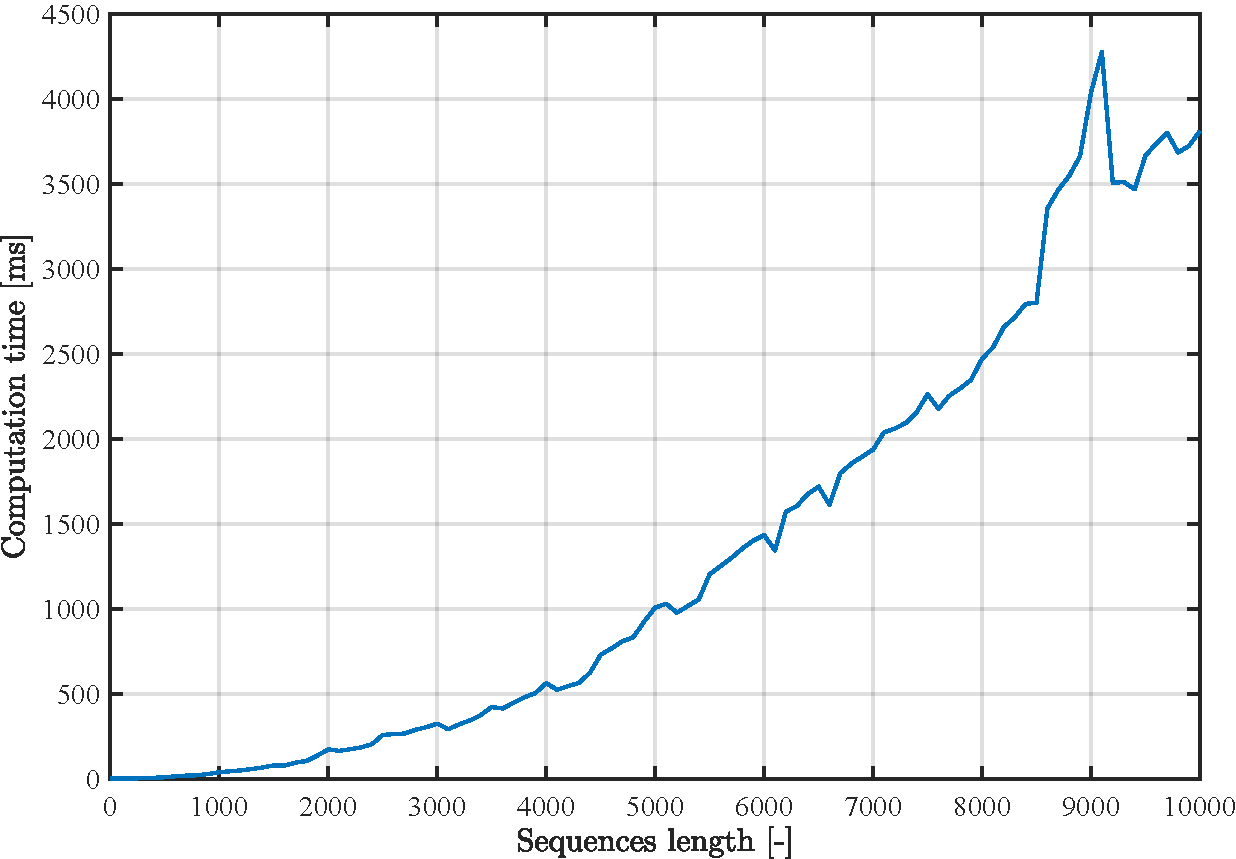
\includegraphics[width=0.65\textwidth]{resources/pdf/dichotomic.pdf}
		\noskipcaption{Évolution du temps de calcul de la recherche dichotomique par force brute en fonction de la taille des séquences.}
		\label{fig:dichotomic}
	\end{figure}
	Or, d'après l'analyse théorique (cf. section \ref{sec:complexity}), la complexité de la recherche dichotomique par force brute devrait être $\mathcal{O}\rbk{m n^2 \log(n)}$. Cependant, si l'on se penche sur les données collectées, il apparaît que le facteur $m$ est quasiment constant. De plus, $\log(n)$ varie assez peu sur l'interval $[0, 5000]$. Il ne serait donc pas étonnant de confondre les deux relations.
	\subsubsection*{Table de hachage}
	Encore une fois, si la courbe comporte beaucoup de bruit\footnote{L'algorithme étant particulièrement rapide, la mesure de son temps de calcul est fort sensible aux perturbations causées par les autres processus du système.}, une relation d'ordre $1$ reste discernable à la Figure \ref{fig:hash}.
	\begin{figure}[H]
		\centering
		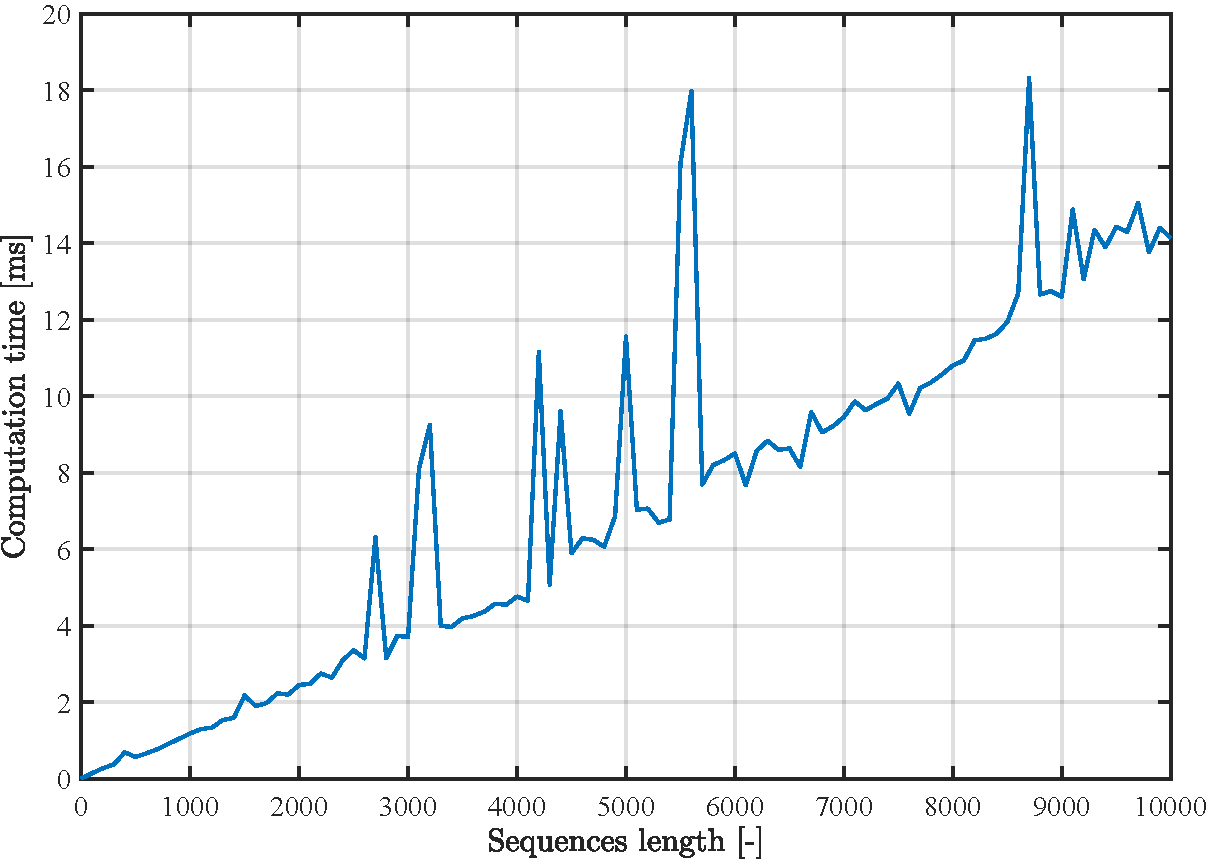
\includegraphics[width=0.65\textwidth]{resources/pdf/hash.pdf}
		\noskipcaption{Évolution du temps de calcul de la recherche dichotomique par table de hachage en fonction de la taille des séquences.}
		\label{fig:hash}
	\end{figure}
	Selon l'analyse théorique, la complexité de la recherche dichotomique par table de hachage (avec calcul incrémental) devrait être $\Theta\rbk{n \log(n)}$. Mais, puisque ici aussi, le facteur $\log(n)$ varie peu sur l'interval $[0, 5000]$, il n'est pas surprenant d'observer ce qui semble être une relation d'ordre $1$.
	\subsubsection*{Programmation dynamique}
	Une fois de plus, une relation d'ordre $2$ est aisément reconnaissable à la Figure \ref{fig:dynamic}.
	\begin{figure}[H]
		\centering
		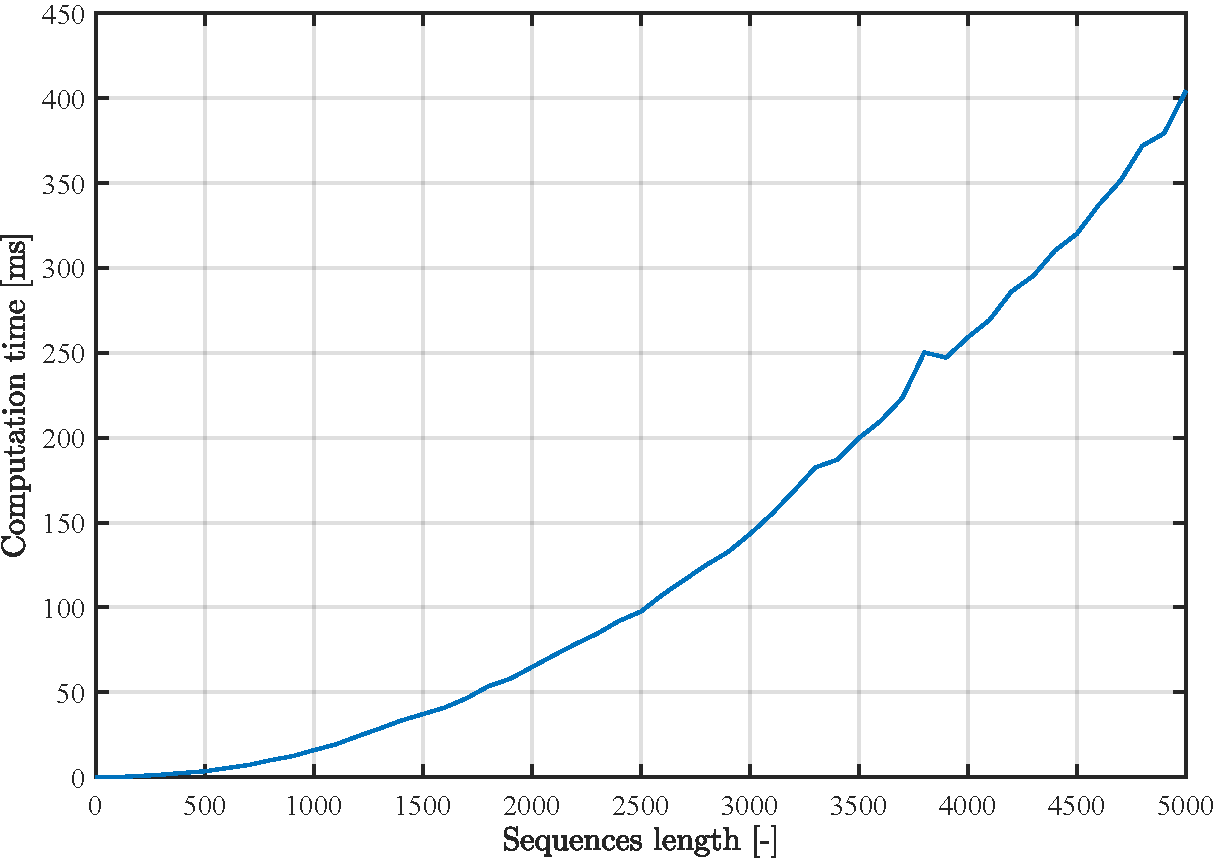
\includegraphics[width=0.65\textwidth]{resources/pdf/dynamic.pdf}
		\noskipcaption{Évolution du temps de calcul de la recherche par programmation dynamique en fonction de la taille des séquences.}
		\label{fig:dynamic}
	\end{figure}
	Cette observation correspond à la complexité théorique, à savoir $\Theta\rbk{n^2}$.
	\newpage
\end{document}
